\documentclass[fleqn]{article}[11pt]
\usepackage{amsmath} 
\usepackage{amssymb}
\usepackage[english]{babel}
\usepackage[autostyle]{csquotes}
\usepackage[margin=0.5in]{geometry}
\newcommand{\ds}{\displaystyle}
\usepackage{graphicx}
\usepackage[oztex]{harpoon}

\begin{document}
	
\begin{center}\section*{MATH 316D W08}\end{center}
\subsection*{DD1 Individual Quiz}

\begin{enumerate}
	
	\item \textbf{Keep}.
	
	\item \textbf{Change} to, ``The following matrix:"
	
		\(\begin{bmatrix}
			1 & 2 & 3 \\
			2 & 4 & 3 \\
			0 & 1 & 6 \\
		\end{bmatrix}\)
			\begin{enumerate}
			 	\item Is row equivalent to the $3\times 3$ identity matrix $I_{3}$.
				\item Is inearly independent about it's columns.
				\item Is invertible.
				\item Has a nonzero determinant.
				\item All of the above. $\implies$ \textbf{Correct}
				\item Only answers \textit{\textup{a}} and \textit{\textup{c}}.
			 \end{enumerate}
	
	\item \textbf{Keep}.
	
	\item \textbf{Keep}.
	
	\item \textbf{Keep}.
\end{enumerate}

\subsection*{DD2 Group Quiz}

\begin{enumerate}
	\item \textbf{Keep}, but please change the format of one of the answers. The answer that needs to be changed is, ``$A$ is row-equivalent to In". Please change to, ``$A$ is row-equivalent to $I_{n}$".
	
	\item \textbf{Keep}.
	
	\item \textbf{Keep}.
	
	\item \textbf{Delete}.
	
	\item \textbf{Keep} (previously question 5).
	
	\item \textbf{Add}, ``Given the following column vectors as shown, what is the area of the parallelogram that they create?"
	
		\begin{figure}[h!]
			\raggedright
				\graphicspath{{/Users/tylertrogden/Desktop/}}
				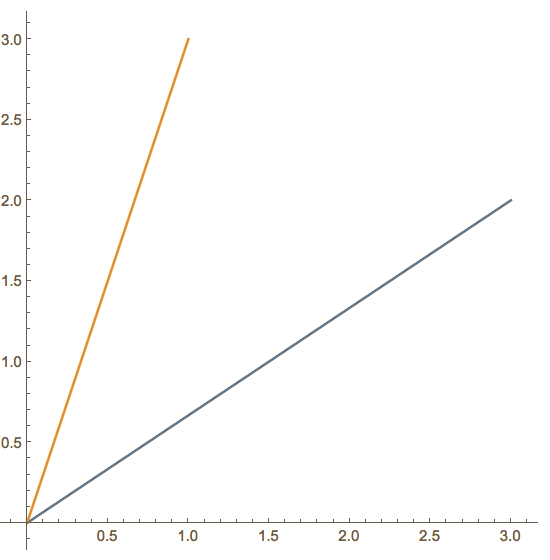
\includegraphics[height=4cm,width=4cm]{W08_GQ_Q4} 
		\end{figure}
			\begin{enumerate}
				\item 11
				\item 3 $\implies$ \textbf{Correct}
				\item -3
				\item Not enough information given.
			\end{enumerate}
	
	\item \textbf{Add}. ``Compute the determinant of the following matrix by hand and select the answer that best represents your work."
	
	$\mathbf{A}$=
	\(\begin{bmatrix}
		1 & -2 & 3 & -4 \\
		0 & 5 & -6 & 7 \\
		0 & 0 & -8 & 9 \\
		0 & 0 & 0 & -10 \\
	\end{bmatrix}\)
	\begin{enumerate}
		\item 0
		\item 246
		\item 400 $\implies$ \textbf{Correct}
		\item -246
		\item The $det(A)$ is not an allowable operation.
	\end{enumerate}
\end{enumerate}

\subsection*{DD3 Weekly Quiz}

\begin{enumerate}
	\item \textbf{Keep} but please reword to, ``If a matrix is a $3\times3$ and has exactly two pivots, then it is possible for the columns of that matrix to span $\mathbb{R}^3$."
	
	\item \textbf{Keep}.
	
	\item \textbf{Keep}.
	
	\item \textbf{Keep}.
	
	\item \textbf{Keep} and please make sure the correct answer keyed is $\implies$ \textbf{False}
	
	\item \textbf{Keep}.
	
	\item \textbf{Change} to what was previously question 8.
	
	\item \textbf{Add}, ``Find the determinant of the following matrix by hand using the method of cofactor expansion about a column, then select the answer that best represents your work."
	
	$\mathbf{A}$=
	\(\begin{bmatrix}
		1 & -2 & 3 & -4 \\
		2 & -5 & -6 & 7 \\
		0 & 4 & -8 & 9 \\
		0 & 0 & 4 & -10 \\
	\end{bmatrix}\)
	\begin{enumerate}
		\item -284 $\implies$ \textbf{Correct}
		\item 0
		\item 400
		\item -400
		\item The $det(A)$ is not an allowable operation.
	\end{enumerate}

	\item \textbf{Keep} but please fix the wording in \textbf{part a.} of the question so that it reads as follows: ``Determine if $\mathbf{v}_3$ is in the span of $\mathbf{v}_1$, and $\mathbf{v}_2$." Also please make sure that appropriate answers are along the lines of: 
	
		\begin{enumerate}
			\item $\overrightharp{v}_3$ is in the span of $\overrightharp{v}_1$ and $\overrightharp{v}_2$ because in RREF the equation $\mathbf{A}\overrightharp{v}=\overrightharp{b}$, where $\mathbf{A}=\{\overrightharp{v}_1, \overrightharp{v}_2\}$ and $\overrightharp{b}=\overrightharp{v}_3$, has a solution. 
			
			\item The vectors in $S$ are not linearly independent, because in RREF vectors $\overrightharp{v}_1$ and $\overrightharp{v}_2$ are linear combinations of $\overrightharp{v}_3$.
			
			\item Yes, the vectors $\overrightharp{v}_1$ and $\overrightharp{v}_2$ span $\mathbb{R}^2$ because these column vectors are linearly independent.
		\end{enumerate}
	
	\item \textbf{Keep}.
\end{enumerate}

\end{document}